\documentclass[a4paper, 12pt]{article}

\usepackage[english]{babel}
\usepackage[utf8x]{inputenc}
\usepackage{amsmath}
\usepackage{graphicx}
\usepackage[hidelinks]{hyperref}

\title{Shadow Volumes using Geometry Shader}
\author{Nora Björklund \and Johan Jönsson}

\begin{document}
\maketitle
\tableofcontents
\newpage
\section{Introduction}
Shadow Volumes is a common way of creating real-time shadows, and has been used
in games such as Doom 3 \cite{gpug1}. In this project the shadow volumes are implemented with the geometry shader. Implementation by geometry shader takes tedious vertex related processing away from the CPU, and insted uses the simultaneous processing power of the GPU.[REF]
\subsection{Project Goal}
\subsection{Planning and Allocation of Work}
\section{Background}
\subsection{Shadow Volumes}
\subsection{Geometry Shader}
\section{Implementation}
\subsection{Program Structure}
\subsection{Object Loader}
In order to produce proper shadow volumes it is necessary to know the neighbours
of each vertex. Passing this information to the shader is a simple process since
OpenGL has built in support for adjacency primitives. All we need to do is
extract the adjacency information for each object, before we upload them to the
shader. This introduces the need for an object loader capable of extracting this
information at the time of loading the objects in the initialization step.

In order to achieve this it was necessary to write a new object loader, more or
less from scratch (inspiration was of course taken from the functions in
loadobj.~c). For this new object loader we decided to use the open source library
assimp (\url{assimp.sourceforge.net}), because of its simplicity and extensive
capabilities.

A short description of how the object loader works, essentially the first step
is to load the object normally, without adjacency information, just like in
loadobj.~c. Once the object has been loaded we create a simple hash table (the
hash function used is in no way even close to being an optimal one, it is merely
a very simple function that gets the job done reasonably well), in which we
insert every pair of indices in every triangle and their corresponding neighbour
in order to allow us to (hopefully) quickly loop through the entire list of all
triangles in the object in order to find the neighbours of each vertex. Once
this is done we simply loop through every vertex in every triangle and look up
the neighbours from the hash table to create a table of every vertex and its
neighbours in order to set up our list of indices for drawing the object..

\begin{figure}[h]
\centering
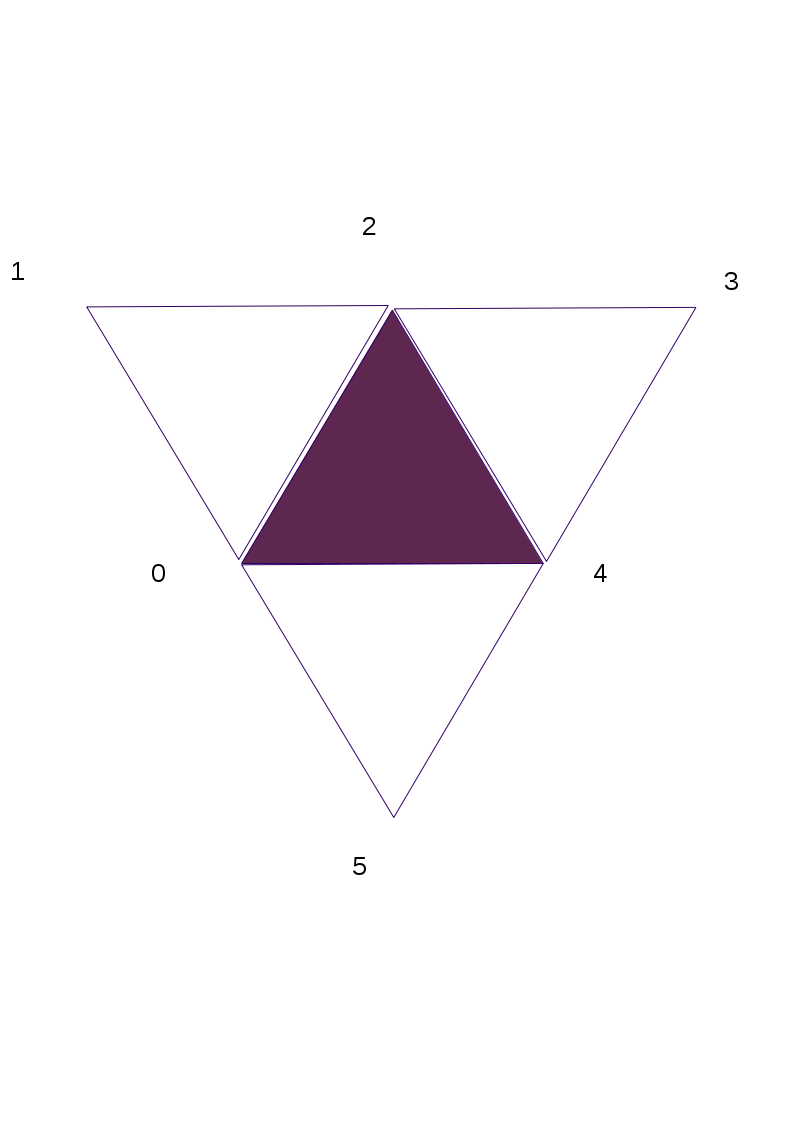
\includegraphics[width=10cm]{triangle_adj.png}
\caption{The triangle with adjacency primitive. Indices 0, 2, 4 form the
original triangle and indices 1, 3, 5 are the adjacent vertices}
\end{figure}

To clarify what the object loader does, first we loop through every triangle in
the object mesh and create a hash table containing the neighbour information for
every them. For the triangle (0,1,2) we begin by inserting the edge (0,1) and
the corresponding neighbour (2), then we insert the edge (1,2) and the
neighbour (0) and finally we insert the edge (2,0) and the neighbour (1). By
doing this for every triangle in the entire model mesh we can simply enter the
edges in any triangle and quickly recover the neighbours of each triangle, e.g.
if we input the edge (2,4) we look in our hash table and find the neighbour
(3). Finally we can construct our list of indices, used for drawing the object,
by looping through every vertex in every triangle and looking up the neighbours.

\subsection{Volumes}
\subsection{Geometry Shader syntax}
\section{Results}
\section{Discussion }


\begin{thebibliography}{9}
\bibitem{gpug1}
	Randima Fernando,
	\emph{GPU Gems: Programming Techniques, Tips and Tricks for Real-Time
	Graphics}.
	Addison-Wesley Professional; First Edition edition, April 1, 2004.
	\url{http://http.developer.nvidia.com/GPUGems/gpugems\_copyrightpg.html}
\end{thebibliography}
\end{document}
